\documentclass[a4paper,12pt]{article}

\usepackage[utf8]{inputenc}
\usepackage{amsmath,amssymb}
\usepackage{geometry}
\usepackage[hypertexnames=false]{hyperref}
\hypersetup{hidelinks}
\usepackage{tikz}
\usepackage{pgfplots}
\pgfplotsset{compat=1.18}
\usetikzlibrary{shapes.geometric,arrows.meta,positioning,fit,calc,backgrounds}
\usepackage[ruled,vlined,linesnumbered]{algorithm2e}
\usepackage{booktabs}
\usepackage{listings}
\usepackage{xcolor}
\usepackage[most]{tcolorbox}
\usepackage{float}
\usepackage{enumitem}
\usepackage{tabularx}

\geometry{margin=1in}
\setlength{\parindent}{0pt}
\setlength{\parskip}{0.6\baselineskip}

% ── Color palette ──
\definecolor{tamblue}{HTML}{2563EB}
\definecolor{tamgreen}{HTML}{059669}
\definecolor{tamorange}{HTML}{D97706}
\definecolor{tamred}{HTML}{DC2626}
\definecolor{tampurple}{HTML}{7C3AED}
\definecolor{tamgray}{HTML}{6B7280}
\definecolor{tmbg}{HTML}{F8FAFC}

% ── Code listing style ──
\lstset{
  basicstyle=\ttfamily\small,
  keywordstyle=\color{tamblue}\bfseries,
  commentstyle=\color{tamgray}\itshape,
  stringstyle=\color{tamgreen},
  backgroundcolor=\color{tmbg},
  frame=single,
  rulecolor=\color{tamgray!30},
  breaklines=true,
  showstringspaces=false,
  language=Python,
}

% ── tcolorbox styles ──
\newtcolorbox{conceptbox}[1][]{
  colback=tamblue!5, colframe=tamblue!60,
  fonttitle=\bfseries, title=#1,
  rounded corners, boxrule=0.5pt
}

\title{\textbf{Tiered Agent Memory (TAM)}\\[6pt]
  \large Multi-tier Cognitive Memory Architecture\\for AI Agents}
\author{minhz99 / tiered-agent-memory}
\date{\today}

\begin{document}
\maketitle

\begin{abstract}
This document presents \textbf{Tiered Agent Memory (TAM)} --- a multi-tier cognitive memory architecture for AI Agents. Unlike traditional RAG systems that only store and retrieve data, TAM simulates the cognitive process: the Agent not only knows how to \emph{remember}, but also how to \emph{ignore} (filter noise), \emph{doubt} (when there are contradictions), \emph{generalize} (see the big picture), and \emph{self-learn} from mistakes. The architecture consists of \textbf{4 storage tiers} (Working, Active, Latent, Archive), \textbf{3 dynamics mechanisms} (Activation, Decay, Reinforcement), and \textbf{7 horizontal control planes} (Query Understanding, Competition, Abstraction, Reasoning, State, Scaling, Evolution). The paper also presents a Python implementation illustrating the full end-to-end 12-step pipeline.
\end{abstract}

\tableofcontents
\newpage

\section{Document Objectives}

This document describes a memory architecture that can be used to design, evaluate, and operate Agents in practice. The core of the architecture remains the 4-tier storage model, but the goal of the document is not just to provide a ``place to remember'', but to clarify the \textbf{memory coordination system}: what is remembered, what is ignored, what should only be activated when cued, what must be doubted, what should be generalized, and what must be converted into reusable reasoning strategies.

If memory is viewed merely as a data warehouse, the system will quickly encounter three problems: retrieval noise, Working Memory bloating, and the generation of ``split personality'' responses when old, new, correct, and incorrect information all crowd into the context. Therefore, a good memory system must simultaneously satisfy four objectives:
\begin{itemize}
    \item \textbf{Contextually correct:} Bringing the right knowledge or the right strategy into the right response turn.
    \item \textbf{Economical:} Keeping Working Memory small enough not to waste tokens and latency.
    \item \textbf{Adaptive:} Allowing memory to change over time, according to new evidence and execution results.
    \item \textbf{Controllable:} Explaining why which memory is selected, which memory is inhibited, which memory is demoted, which memory is marked obsolete, and which memory is elevated into a general strategy.
\end{itemize}

The current architecture is on the right track thanks to stratification, Latent Memory, trigger-based recall, competition, abstract memory, and intent-based gating. However, to truly reach the production-ready level and become closer to human memory, the system needs four core upgrades:
\begin{itemize}
    \item \textbf{Reasoning Memory:} Storing generalizable problem-solving strategies, rather than just facts or events.
    \item \textbf{Contrastive Signals:} Learning not only from successes but also from failure trajectories and dead ends.
    \item \textbf{MaTTS (Memory-aware Test-Time Scaling):} When the budget is high, the system not only retrieves deeper but also expands multi-branch reasoning guided by memory.
    \item \textbf{Self-Evolving Background Worker:} A background worker that not only cleans up memory but also curates logs into higher-quality memories and injects them back into Active Memory.
\end{itemize}

In short: the current system already ``knows how to remember'', but to truly become more powerful it must also learn how to ``reason again, learn from mistakes, scale at the right time, and self-evolve''.

\section{Overall Model: 4 Tiers + 3 Mechanisms + 7 Control Planes}

The architecture should be understood as three overlapping layers.

The first layer is the \textbf{four storage tiers}, answering the question \emph{where does memory reside and what is its availability level}. These four tiers are:
\begin{itemize}
    \item \textbf{Working Memory (WM):} The active context layer in the current request.
    \item \textbf{Active Memory:} The stable, fast-access knowledge layer, which is the default retrieval source.
    \item \textbf{Latent Memory:} The infrequently used memory layer, only activated when there is a strong enough cue.
    \item \textbf{Archive:} The cold storage layer, serving tracing, offline analysis, and rare recovery.
\end{itemize}

The second layer is the \textbf{three dynamics mechanisms}, answering the question \emph{how does memory surface, fade, or become strengthened}. These three mechanisms are:
\begin{itemize}
    \item \textbf{Activation:} The mechanism that makes a memory or a strategy a candidate for the current reasoning turn.
    \item \textbf{Decay:} The mechanism that reduces the probability of a memory being selected over time, by memory type, and by the level of disuse.
    \item \textbf{Reinforcement:} The mechanism that consolidates memories that have been used and proven useful.
\end{itemize}

The third layer is the \textbf{seven horizontal control planes} -- deciding whether the architecture is truly production-ready and close to human memory. These seven planes are:
\begin{itemize}
    \item \textbf{Query Understanding Plane:} Intent classification, query rewriting, cue expansion.
    \item \textbf{Competition Plane:} Competition, inhibition, dedup, and selection among competing memories.
    \item \textbf{Abstraction Plane:} Creating abstract memories and extracting general principles.
    \item \textbf{Reasoning Plane:} Managing Reasoning Memory and ReasoningBank as a repository of reusable strategies.
    \item \textbf{State Plane:} Managing conflicts, validity time, currency, and forgetting strategies by memory type.
    \item \textbf{Scaling Plane:} Managing MaTTS, i.e., memory-guided test-time scaling.
    \item \textbf{Evolution Plane:} Managing contrastive signals, reflection, and self-curation in the background worker.
\end{itemize}

The key point is: \textbf{the 4 tiers are just the storage topology}. For the system to be more ``human-like'' and practical to use, control planes are needed so that it not only knows how to remember but also knows how to choose strategies, learn from mistakes, expand reasoning when needed, and rewrite memories at a higher quality level.

\section{Core Design Principles}

\subsection*{Principle 1: Memory is an activation system, not a storage warehouse}

A larger warehouse does not mean a better memory system. The quality of memory must be measured by the ability to activate the right knowledge or strategy at the right time, not by the number of records stored.

\subsection*{Principle 2: Queries must be re-interpreted before retrieval}

Humans rarely access memory using the exact words just heard. The brain often reinterprets the question into adjacent concepts. Therefore, a good Agent should not retrieve directly from the original query but should have a \emph{query rewriting/query expansion} step to expand from the surface text to concepts that are truly useful for recall.

\subsection*{Principle 3: Memories must compete, not just be ranked}

Taking the top-$K$ by score is not enough. Related memories must \textbf{compete} to be activated, and a stronger memory must be able to \textbf{inhibit} similar or redundant memories. Without competition/inhibition, the system will often bring into WM many memories that are identical or almost correct but wrong in context.

\subsection*{Principle 4: The system must have atomic, abstract, and reasoning memory}

Atomic memory is great for storing a specific detail. Abstract memory is great for grasping the ``big picture''. But for the Agent to truly learn how to solve new tasks, \textbf{Reasoning Memory} is needed -- that is, the layer that stores problem-solving strategies that can be reused across different situations.

\subsection*{Principle 5: The system must learn from both successes and failures}

If reinforcement only rewards what was done correctly, the system misses half the important lessons. Dead-end trajectories, trial-and-error branches, and ineffective strategies are highly valuable \textbf{contrastive signals} to extract sharper principles.

\subsection*{Principle 6: Time, conflict, and currency are first-class properties}

A memory not only needs to be correct in content; it also needs to be correct regarding \emph{when}. Without temporal awareness and conflict resolution, the system easily retains states or strategies that have expired.

\subsection*{Principle 7: Intent is just as important as domain}

Domain gating is necessary, but not sufficient. A personal memory about the gym might share a broad domain with a question about optimizing a diet, but it is entirely unnecessary if the current intent is analyzing an algorithm. Therefore, memory usage must be filtered by \textbf{intent}, not just by domain.

\subsection*{Principle 8: Not all types of memory forget the same way}

Episodic memory should be forgotten faster than semantic memory; reasoning memory should only weaken when that strategy is counter-exemplified or no longer effective; system memory should almost never undergo decay by the same mechanism as episodic memory.

\subsection*{Principle 9: High budget must scale reasoning, not just retrieval}

Old-style attention budgets answer the question ``how many memory tiers to open''. MaTTS goes further: when the problem is hard, a high budget must activate multi-branch reasoning, sequential or parallel, guided by memory to avoid blind exploration.

\subsection*{Principle 10: Self-evolution should be the background worker's responsibility}

The online path must be fast, neat, and safe. Heavy work like reading all daily logs, comparing successes with failures, synthesizing general principles, and rewriting higher-quality memories should be delegated to a background worker.

\section{Tier 1: Working Memory --- The Current Thinking Space}

\subsection*{System Role}

Working Memory is the context portion that the model sees in the current response turn. With LLMs, this is where the highest operational power lies: what is not brought into the WM is almost entirely unable to directly affect the response.

WM is not a place to ``store'' but a place to \textbf{compose}. It should be built from five main sources:
\begin{itemize}
    \item The current request.
    \item The short-term history of the conversation.
    \item The system instructions currently in effect.
    \item A small set of memories that have gone through query rewrite, retrieval, competition, conflict filtering, and compression.
    \item Control parameters such as recall confidence, strategy hints from ReasoningBank, and the current scaling mode of MaTTS.
\end{itemize}

\subsection*{Minimum Specification}

A good WM should follow these rules:
\begin{itemize}
    \item \textbf{Budget cap:} The memory part only occupies a small fraction of the total context.
    \item \textbf{Small top-$K$:} Only keep the very best candidates.
    \item \textbf{Competition before injection:} Do not allow many similar memories into WM at the same time.
    \item \textbf{Atomic + abstract + reasoning mix:} When appropriate, prioritize a small mix of details, generalizations, and strategies instead of many disjointed pieces.
    \item \textbf{Intent-aware gating:} If the current intent is technical, avoid pulling irrelevant personal memories.
    \item \textbf{Meta-memory:} If recall confidence is low, WM must reflect that uncertainty rather than presenting the memory as an absolute truth.
    \item \textbf{Budget-aware reasoning:} If MaTTS is in a high scaling mode, WM needs to leave room for reasoning branches and guiding strategies.
\end{itemize}

\subsection*{Core Trade-off}

The central trade-off of WM is not only between ``a lot of information'' and ``few tokens'', but also between \textbf{detail}, \textbf{generalization}, and \textbf{strategy}. Introducing too many atomic memories will make WM heavy and confusing; introducing abstract memory too early can lose important details; introducing overly general strategies can make the response ``purely theoretical''. Therefore, WM should always be viewed as a controlled mix of detailed representations, generalized representations, and strategy hints.

\section{Tier 2: Active Memory --- Stable Knowledge, Default Access}

\subsection*{System Role}

Active Memory contains knowledge with a high probability of reuse: semantic memory, style profile, system memory, and verified Reasoning Memories. These are what the Agent should ``think of by default'' first.

\subsection*{Criteria for a Memory to be in Active}

A memory should only reside in Active if it satisfies most of the following conditions:
\begin{itemize}
    \item Has relative stability.
    \item Useful for many future turns.
    \item Has clearly defined domain and intent scopes.
    \item Has high reliability.
    \item Can be represented compactly.
    \item Is not just a short-term state that is about to expire.
    \item If it is a strategy, there must be evidence that it has helped solve a class of problems, not just a single case.
\end{itemize}

\subsection*{Retrieval Mechanism}

Retrieval from Active should be the default, but not \emph{always-include}. Active only provides candidates. Afterwards, the candidate still has to pass the intent filter, competition, conflict filter, and budget filter before being allowed into WM.

Within Active, at least four families of memories should be separated:
\begin{itemize}
    \item \textbf{Semantic/personal memory:} User preferences, roles, constraints.
    \item \textbf{System memory:} Policies, environment, tool capabilities.
    \item \textbf{Style memory:} Preferences for length, tone, response structure.
    \item \textbf{Reasoning memory:} Problem-solving strategies that have been generalized and verified.
\end{itemize}

\subsection*{Core Trade-off}

The biggest risk of Active is not only \textbf{over-personalization}, but also \textbf{over-trusting old strategies}. A reasoning strategy that was once correct in many cases can still become wrong when the context changes. Therefore, reasoning memory in Active must be accompanied by a clear validity scope and validation state.

\section{Tier 3: Latent Memory --- Dormant Memories Requiring Activation Cues}

\subsection*{System Role}

Latent Memory stores episodic memory, transient strategies, reasoning traces, and infrequently used details that still have potential value: old incidents, short-term habits, past projects, symptoms previously mentioned, strategies tried, and dead-end trajectories.

\subsection*{Activation Principles}

Latent should not be accessed by default in every turn. It should only activate when there is a strong enough cue after the query rewriting step. These cues can come from:
\begin{itemize}
    \item \textbf{Keyword cue:} Exact or near-exact match of important keywords.
    \item \textbf{Semantic cue:} The new query is semantically close to an old experience.
    \item \textbf{Explicit cue:} The user explicitly asks to recall something.
    \item \textbf{Risk cue:} The current problem has a high risk if an old memory is missed.
    \item \textbf{Strategy cue:} The current problem is similar to a family of problems where the system previously succeeded or failed.
\end{itemize}

\subsection*{Two-pass retrieval as default specification}

A reasonable process is:
\begin{enumerate}
    \item Pass 1: The rewritten query is used to fetch candidates from Active and ReasoningBank.
    \item Pass 2: If the trigger is strong enough, the expanded query continues to be used to fetch candidates from Latent.
\end{enumerate}

The new point to emphasize is: \textbf{the query for Latent should not be the original query}. It should be the re-interpreted query to increase recall. This is a huge difference between ``having latent memory'' and ``using latent memory effectively''.

\subsection*{Core Trade-off}

Latent allows the system to recall rare things, but it is also the place most prone to false activation. Therefore, Latent always needs to be accompanied by competition, inhibition, recall confidence, and contrastive filtering. The system not only needs to ask ``which memories are related'', but also ``which memory is worth trying again'' and ``which failed memory should be used as a warning instead of advice''.

\section{Additional Layer: Abstract Memory --- The Generalization Layer to Reduce Tokens and Increase Understanding}

\subsection*{Why it is needed}

An architecture with only atomic memory will be very clean in terms of retrieval, but lacks a layer of generalization. When the user has many small memories centered around a topic, the system needs a high-level representation to capture the ``big picture'' without loading too many details into WM.

For example, atomic memories like ``likes gym'', ``once asked about diet'', ``often asks about calories'' can be merged into an abstract memory: ``User cares about health and fitness.''

\subsection*{Architectural Nature}

Abstract Memory doesn't necessarily have to be an independent ``fifth storage tier'' separate from the original 4 tiers. The more correct way is to view it as a \textbf{horizontal synthesis layer} running on top of Active and Latent. It is created by merging related memories and is used primarily for:
\begin{itemize}
    \item Token-saving context injection.
    \item Maintaining consistent thematic continuity.
    \item Increasing reasoning ability at a generalized level.
    \item Acting as a representative in competition when many atomic memories on the same topic compete.
    \item Serving as a premise to distill Reasoning Memory from many individual cases.
\end{itemize}

\subsection*{Core Trade-off}

Abstract memory helps reduce tokens and increase coherence, but if abstraction happens too early, the system loses important details. Thus, abstract memory should be viewed as a \textbf{supplementary} layer, not a complete replacement for atomic memory.

\section{Additional Layer: Reasoning Memory and ReasoningBank}

\subsection*{Why it is needed}

The existing memory tiers mainly answer the question ``What does the Agent know about the user, the system, and the past?''. But for the Agent to carry skills from an old task to a new task, an additional layer is needed to answer a different question: \textbf{``What problem-solving strategies has the Agent learned?''}

Reasoning Memory does not store ``knowledge'' in the sense of a single fact, but stores \textbf{Generalizable Reasoning Strategies}. For example, instead of just remembering that a specific bug was fixed in which commit, it stores the principle: ``When encountering error X in module Y, check the config file Z first because there are often asynchronous errors.'' This type of memory has a much higher ability to generalize than episodic memory.

\subsection*{Where does it sit in the architecture}

Operationally, Reasoning Memory sits at the intersection of Active and Abstract:
\begin{itemize}
    \item It belongs to \textbf{Active} because it must be accessed quickly when encountering similar problems.
    \item It belongs to \textbf{Abstract} because its nature is the generalized result of many experiences.
    \item The raw trajectories that generated that strategy might reside in \textbf{Latent} or \textbf{Archive}.
\end{itemize}

Therefore, a reasonable implementation is to have a \textbf{ReasoningBank} as a sub-bank of Active/Abstract, which contains validated strategies.

\subsection*{Core Trade-off}

Reasoning Memory is very powerful because it helps the Agent not have to ``reinvent how to think'' for each new task. But it is also dangerous if the strategies are distilled from too few examples or from an overly narrow context. Therefore, reasoning memory must be attached to an \textbf{applicability scope}, \textbf{validation status}, and \textbf{contrastive evidence} rather than just a beautiful summary sentence.

\section{Tier 4: Archive --- Cold Storage, Serving Deep Retrieval}

\subsection*{System Role}

Archive holds full history, snapshots, raw traces, successful and failed trajectories, and data for auditing or offline analysis. This is where the problem of ``storing to survive'' is solved, not a place for permanent reasoning.

\subsection*{Operational Specification}

The Archive should have:
\begin{itemize}
    \item Minimal indexing by time, user, domain, event type, and trajectory type.
    \item Snapshot summaries for fast re-hydration.
    \item Clear retention policies.
    \item Ability to selectively extract up to Latent, Active, or ReasoningBank when needed.
    \item Clear links so the worker can trace back successful and failed raw trajectories for the self-curate step.
\end{itemize}

\subsection*{Core Trade-off}

An Archive without indexing or snapshot summaries is just a log dump. The value of Archive does not lie in ``keeping a lot'', but in \textbf{being able to recover the right things when needed at an acceptable cost}, and recovering both the right and the wrong to serve contrastive learning.

\section{State Specification of a Memory}

For the architecture to be truly deployable, each memory needs a minimum state rich enough to support retrieval, conflict resolution, temporal awareness, reasoning transfer, and explainability. A minimal record should carry the following groups of properties:
\begin{itemize}
    \item \textbf{Identity:} ID, storage tier, and memory type.
    \item \textbf{Content:} Content summary, abstraction group if any, and if it's a reasoning memory, the core strategy and application scope.
    \item \textbf{Context:} Domain tags, intent tags, module tags, or task family if needed.
    \item \textbf{Source and Reliability:} Origin of the memory, confidence, recall confidence, and verification state.
    \item \textbf{Time:} Validity start time, validity end time, currency flag, creation time, last verified time, and last used time.
    \item \textbf{Behavior:} Usage count, reinforcement score, decay profile.
    \item \textbf{Contrastive Evidence:} References to success cases, failure cases, causes of failure, and reflection summaries.
    \item \textbf{Conflict:} Conflict status, which memory it replaces or is replaced by.
\end{itemize}

Not every memory needs to have all fields fully populated, but without these groups of properties, the system will have a hard time solving the problem of ``which memory is correct, still valid, reliable, transferable, and should be chosen right now''.

\section{End-to-End Data Flow Specification}

A production-ready processing turn should be described as a twelve-step pipeline.

\subsection*{Step 1: Intent, domain, and complexity analysis}

The system determines what kind of question the user is asking: technical, personal, retrospective, decision-making, or simple. This is the first step that decides which memories are allowed to participate and whether the task requires test-time scaling.

\subsection*{Step 2: MaTTS budget setup}

Instead of just deciding ``how many memory tiers to open'', the system determines the scale of reasoning at runtime. If the query is simple, the system takes the fast path: minimal retrieval, no multi-branch expansion. If the query is difficult, ambiguous, or high risk, the system turns on \textbf{MaTTS} to allow deeper sequential or parallel reasoning.

\subsection*{Step 3: Query rewriting / query expansion}

The user's original query is re-interpreted into concepts better suited for memory retrieval. This expands the surface language into concepts useful for retrieval and for selecting strategies in the ReasoningBank.

\subsection*{Step 4: Intent-aware gating}

Before searching for memories, the system eliminates memory families incompatible with the intent. For example, if the intent is algorithm explanation, a personal memory about the gym shouldn't compete even if they share a broad ``self-improvement'' domain.

\subsection*{Step 5: Background retrieval from Active and ReasoningBank}

The rewritten query is used to search Active via vector search, metadata filtering, and domain filtering. Simultaneously, the system queries ReasoningBank for strategies that succeeded in similar problem families.

\subsection*{Step 6: Latent cue detection}

The system checks if there are keyword cues, semantic cues, explicit cues, risk cues, or strategy cues strong enough to open Latent.

\subsection*{Step 7: Expanded retrieval from Latent, Abstract Memory, and raw traces}

If cues exceed the threshold, the system uses query expansion to search Latent. Also, if multiple atomic memories of the same topic appear, the system might retrieve abstract memories representing that group. For very hard queries, it might also fetch trace summaries from Archive to provide context for reflection or branch guidance.

\subsection*{Step 8: Competition, inhibition, and conflict filtering}

Candidates are not just ranked by score, but \textbf{compete}. Stronger memories can inhibit near-duplicates or less useful ones. Conflicting memories must be flagged or de-prioritized before entering WM.

\subsection*{Step 9: Working Memory construction}

WM is built from a small mix of atomic memories, abstract memories, reasoning memories, and control parameters like style overrides or recall confidence. If recall confidence is low, the system should prepare phrasing reflecting uncertainty rather than over-asserting.

\subsection*{Step 10: MaTTS activation and multi-branch reasoning}

If the budget is high enough, the system does not stop at a single reasoning pass but activates \textbf{Memory-aware Test-Time Scaling}. Here, the Agent might run reasoning branches sequentially or in parallel, similar to Tree of Thoughts, but not blindly: ReasoningBank provides strategy hints to guide exploration more efficiently.

The correct relationship here is:
\begin{itemize}
    \item \textbf{Memory guides Scale:} Old strategies keep new branches from wandering.
    \item \textbf{Scale feeds back to Memory:} New branches create various solution paths, both right and wrong, providing data for contrastive learning.
\end{itemize}

\subsection*{Step 11: Answer selection, recording successes and failures}

After reasoning branches finish, the system selects the final answer based on intrinsic quality, consistency, and confidence. More importantly, it does not only record the winning branch. Losing branches, dead ends, and causes of failure are also kept as \textbf{contrastive signals}.

\subsection*{Step 12: Update, reflection, and self-evolution schedule}

After generation, the system updates reinforcement for useful memories, applies decay by memory type, marks conflicts as outdated, updates validity time on state changes, and creates a \textbf{reflection summary} like: ``Strategy A succeeded, Strategy B failed because cause C.'' This reflection serves short-term updates and is queued for the background worker to distill later.

\section{Upgraded Operational Mechanisms}

\subsection*{Activation + Competition}

Activation should not just be adding similarity, importance, recency, and confidence. It needs a \textbf{competition} component. A memory is selected not only because it is strong, but because it beats near-duplicates or direct competitors.

Competition prevents two common errors:
\begin{itemize}
    \item Many similar memories crowding into WM causing noise.
    \item Almost-correct but out-of-context memories winning due to high similarity.
\end{itemize}

\subsection*{Decay + Forgetting by Memory Type}

Decay must depend on the type of memory. A reasonable profile is:
\begin{itemize}
    \item \textbf{Episodic memory:} Fast decay.
    \item \textbf{Semantic memory:} Slow decay.
    \item \textbf{Reasoning memory:} Slow decay but sensitive to counter-examples and failure signals.
    \item \textbf{Style/profile memory:} Medium decay and depends on recent confirmations.
    \item \textbf{Skill/system memory:} Almost no decay by the same mechanism as episodic.
\end{itemize}

\subsection*{Reinforcement + Contrastive Signals}

Reinforcement shouldn't just increase scores for what was ``done right''. The system must learn from both successful and failed experiences. Dead-end trajectories shouldn't be completely discarded; they should be kept as \textbf{contrastive signals} helping the system distinguish between ``strategies to try again'' and ``strategies to avoid''.

A good reflection doesn't just say ``Approach A is effective'', but goes further: ``A is more effective than B because B fails when assumption C is false.'' This contrast is what creates sharp reasoning memory.

\subsection*{Reasoning Memory Formation}

Reasoning Memory is formed when the system distills multiple traces into a generalizable, transferable strategy. Crucially, it must not be generated from a single case if that case is not representative enough. A strategy should only be pushed to ReasoningBank when:
\begin{itemize}
    \item It has appeared or been confirmed in multiple situations.
    \item Its applicability scope is clear.
    \item There is contrastive evidence showing why it is better than competing strategies.
\end{itemize}

\subsection*{Conflict Resolution}

This is a mandatory mechanism to avoid ``split personalities''. When a new memory conflicts with an old one, the system must have a clear policy:
\begin{itemize}
    \item Reduce the confidence of the old memory.
    \item Mark the old memory as outdated or superseded.
    \item Only keep the old memory in Latent/Archive if it still has historical value.
    \item Do not allow both into WM as two current truths.
    \item If the conflict is at the strategy level, explicitly note which strategy is counter-exemplified by the new case.
\end{itemize}

\subsection*{Temporal Awareness}

Recency and TTL are not enough. The system needs to distinguish between \textbf{current memory} and \textbf{formerly true memory}. For reasoning memory, temporal awareness must also answer: is this strategy still relevant, or only true for an older system version, configuration, or environment.

\subsection*{Meta-memory}

Meta-memory is the ability to know ``I don't remember for sure'' or ``I have an old strategy, but I'm not sure if it still applies''. This step brings the system closer to human memory. If recall confidence is low, the response should use frames like: ``I'm not entirely sure, but it seems that in the past...'' instead of presenting the memory as an absolute fact.

\subsection*{MaTTS: Memory-aware Test-Time Scaling}

MaTTS is a direct upgrade to Attention Budget. Instead of just deciding whether to turn latent retrieval on or off, MaTTS decides the \textbf{scaling level of the reasoning process}. When the task is hard, the system can:
\begin{itemize}
    \item Increase the number of reasoning branches.
    \item Run sequentially or in parallel.
    \item Use ReasoningBank to orient the branches.
    \item Compare trajectories to generate new contrastive evidence.
\end{itemize}

Thus, MaTTS is not just a token-saving strategy. It is the mechanism that allows memory and reasoning to act symbiotically.

\section{Rules for Creating, Updating, Promoting, and Self-Evolving}

\subsection*{Creation}

Not every utterance should be saved. A good write path evaluates:
\begin{itemize}
    \item The clarity of the utterance.
    \item The expected durability.
    \item The value for future turns.
    \item The domain and intent scope.
    \item The potential for conflict with existing states.
    \item The memory type to be assigned if saved.
    \item Whether this is just an isolated experience or has enough substance to be distilled into reasoning memory.
\end{itemize}

\subsection*{Reflection from Successes and Failures}

After hard tasks, the system should generate short reflections answering three questions:
\begin{itemize}
    \item Which strategy succeeded.
    \item Which strategy failed.
    \item Did the failure stem from false assumptions, missing information, or misapplication of context.
\end{itemize}

This reflection bridges raw trajectories and Reasoning Memory.

\subsection*{Promotion}

A memory should be elevated from Latent to Active when it is not only recalled multiple times but also demonstrates stability, few conflicts, and high reuse value. For reasoning memory, promotion demands more: the strategy must prove its ability to generalize across multiple tasks, not just a single case.

\subsection*{Demotion}

A memory in Active should be demoted to Latent when it is no longer frequently used, no longer a default priority, or has lost its currency but remains worth keeping as historical context. For reasoning memory, demotion occurs when a once-useful strategy meets many new counter-examples.

\subsection*{Archiving}

Very old memories with low recall and almost no value for daily reasoning should be moved to Archive. But archiving doesn't mean deleting. It is moving from ``hot reasoning'' to ``cold storage'', while still retaining raw materials so the worker can re-synthesize when needed.

\subsection*{Self-Evolving Background Worker}

This is the part that helps the architecture truly ``evolve''. The background worker should do more than garbage collection. Periodically, it must:
\begin{itemize}
    \item Gather all logs and trajectories of daily tasks.
    \item Separate success and failure cases.
    \item Call an LLM acting as a \textbf{Synthesizer} to analyze why the Agent failed at one task but succeeded at another today.
    \item Distill general principles into higher-quality memories.
    \item Inject the best memories back into Active Memory or ReasoningBank after passing a validation gate.
\end{itemize}

This is when the system transitions from maintenance to \textbf{self-curation}. That is, not only keeping memory cleaner but also making memory smarter over time.

\section{Style Memory and Context Override}

The style profile is a very useful part of Active Memory, but style should not be a hard rule. It must be adjusted by the current context. A reasonable way to think about it is:
\[
\text{final\_style} = 0.7\,\text{user\_style} + 0.3\,\text{context\_style}
\]

The specific coefficients are just illustrative. The important point is: the user's preferred style should be respected, but when the current task is technical analysis, mathematical proof, or production bug handling, the context style must have the authority to pull the response toward rigor.

\section{Cost, Performance, and Scalability Optimization}

The most important optimization levers of this upgraded system are:
\begin{itemize}
    \item \textbf{Adaptive MaTTS:} Only scale multi-branch reasoning when truly necessary.
    \item \textbf{Conditional query expansion:} Only expand deeply when there are signs of latent recall or high risk of omission.
    \item \textbf{Competition before injection:} Reduce the number of topically redundant memories entering WM.
    \item \textbf{Abstract memory:} Reduce tokens while preserving the ``big picture''.
    \item \textbf{Reasoning memory:} Reuse strategies instead of rediscovering from scratch on every task.
    \item \textbf{Contrastive logging:} Turn failures into training data rather than lost costs.
    \item \textbf{Background self-curation:} Move heavy synthesis work to the worker, keeping the online path neat and fast.
\end{itemize}

A production-ready system isn't one that always ``thinks the deepest'', but one that knows when to think deeply, when to use old strategies, when to expand multi-branches, and when to let the background worker synthesize the lessons.

\section{Common Design Errors}

\subsection*{Error 1: Only having top-$K$ without competition}

This allows many similar memories to enter WM, or almost-correct but out-of-context memories aren't strongly inhibited.

\subsection*{Error 2: Retrieving directly from the original query}

Latent Memory exists but recall is very weak because the system does not reinterpret the question into necessary concepts.

\subsection*{Error 3: Only having atomic memory without abstract memory}

The system either has to load many small fragments into WM or loses the ability to grasp the big picture of the user and the situation.

\subsection*{Error 4: No Reasoning Memory}

The Agent only knows facts and old experiences but cannot truly transfer ``problem-solving strategies'' from one task to another.

\subsection*{Error 5: Only learning from successes and ignoring failures}

The system continuously rewards what was right but never clearly understands why other reasoning paths were wrong, leading to shallow strategy learning and repeated dead ends.

\subsection*{Error 6: No conflict resolution}

Old and new memories coexist as two current truths, leading to contradictory responses.

\subsection*{Error 7: No temporal awareness}

The system fails to distinguish between ``is currently like this'' and ``used to be like this'', or ``strategy that used to be useful'' and ``strategy that is still relevant''.

\subsection*{Error 8: Budget only controls retrieval without scaling reasoning}

High-budget mode just spends tokens finding more memories, but the Agent still thinks along a single path and misses the benefits of test-time scaling.

\subsection*{Error 9: Background worker only cleans up without self-curation}

The system might get cleaner over time, but not truly smarter over time.

\subsection*{Error 10: No meta-memory}

The Agent appears either ``certain'' or ``ignorant'' without being able to express a reasonable state of uncertainty.

\section{Evaluation Criteria for a Practical Memory System}

To evaluate this system in production, the following questions should be asked:
\begin{itemize}
    \item Does query rewriting actually increase latent recall without overly inflating false recall?
    \item Does competition reduce redundancy in WM?
    \item Does abstract memory help reduce tokens while maintaining the major topic?
    \item Does reasoning memory help transfer strategies from old tasks to new ones?
    \item Do contrastive signals truly make reflections sharper?
    \item Does conflict resolution prevent contradictory memories from both being considered current?
    \item Does temporal awareness correctly distinguish between current and past states?
    \item Does MaTTS improve quality on hard queries without causing costs to explode on simple ones?
    \item Does the background worker create truly useful higher-quality memories or just generate more noise?
    \item Is recall confidence well-calibrated enough so that responses reflect appropriate uncertainty?
\end{itemize}

A good system not only answers well but must allow the designer to see why it chose to remember this, ignore that, doubt the other, learn from which mistake, and distill what new principle.

\section{Core Conclusion}

The current 4-tier architecture is on the right track because it already knows how to \textbf{stratify}, has \textbf{Latent Memory}, has \textbf{trigger-based recall}, has \textbf{competition}, and has \textbf{abstract memory}. That is the ``knowing how to remember'' and ``knowing how to choose'' part of the system.

But to be truly close to human memory and robust enough for production, the architecture needs to implement the next four core upgrades:
\begin{itemize}
    \item \textbf{Reasoning Memory / ReasoningBank:} So the Agent knows not just facts, but strategies.
    \item \textbf{Contrastive Signals:} So the Agent learns from both successes and failures.
    \item \textbf{MaTTS:} So a high budget doesn't just open more memories but scales guided multi-branch reasoning.
    \item \textbf{Self-Evolving Background Worker:} So the system is not only cleaned up but also self-curates and self-evolves.
\end{itemize}

If the entire specification had to be summarized in one short sentence, it would be: \textbf{a good memory system not only knows how to remember, but also knows how to extract strategies, learn from mistakes, and rewrite its own memory}. These three capabilities are what take the 4-tier architecture from the level of ``conceptually correct'' to the level of ``sharp enough to run for real and alive enough to self-evolve''.

%% ══════════════════════════════════════════════════════════════
%% APPENDIX: DIAGRAMS, TABLES, ALGORITHMS, AND SOURCE CODE
%% ══════════════════════════════════════════════════════════════

\appendix
\newpage

\section{Overall Architecture Diagram}

\begin{figure}[H]
\centering
\resizebox{\textwidth}{!}{%
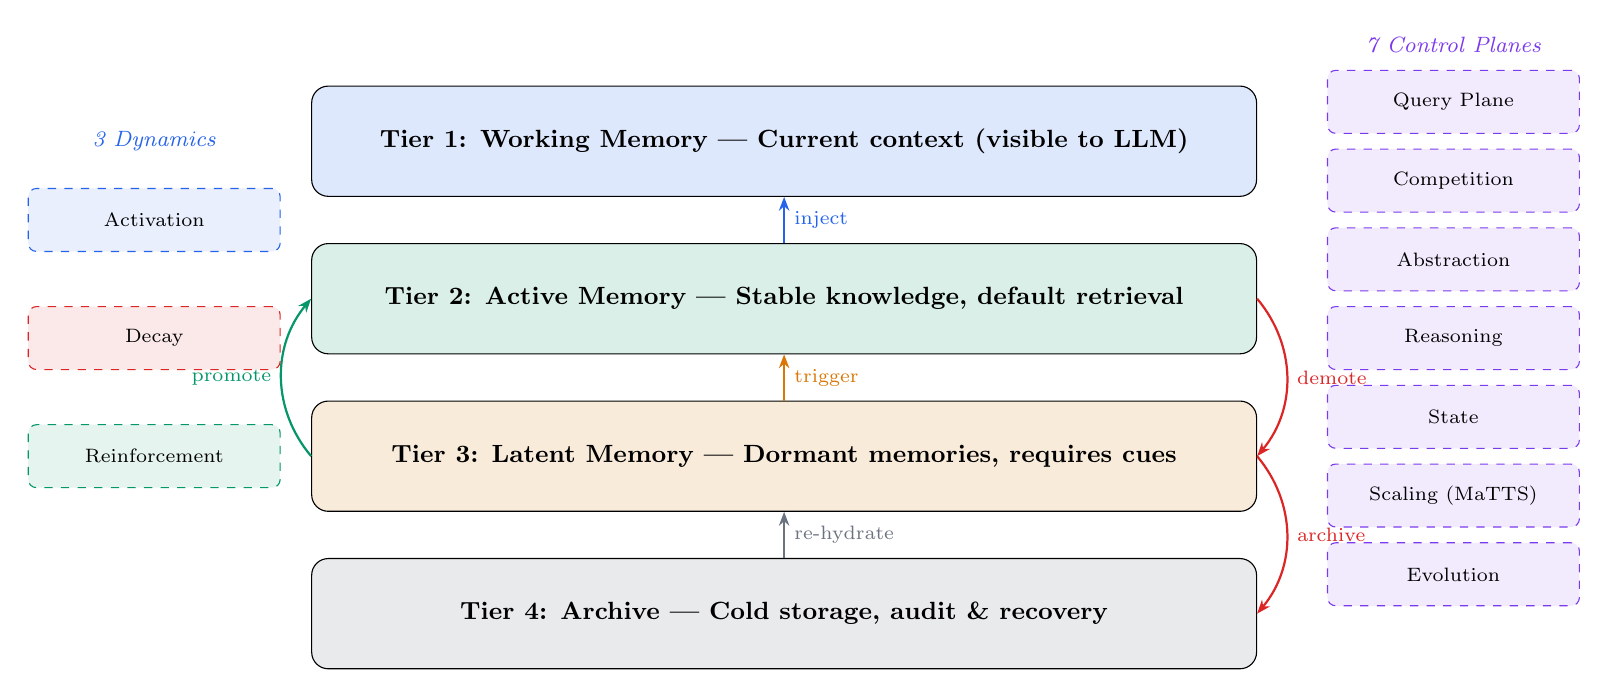
\begin{tikzpicture}[
  tier/.style={draw, rounded corners=6pt, minimum width=12cm, minimum height=1.4cm, font=\small\bfseries, align=center},
  plane/.style={draw, dashed, rounded corners=3pt, minimum width=3.2cm, minimum height=0.8cm, font=\scriptsize, align=center},
  arrow/.style={-{Stealth[length=5pt]}, thick},
  every node/.style={font=\small},
]
% Tiers (bottom to top)
\node[tier, fill=tamgray!15] (archive) at (0,0) {Tier 4: Archive --- Cold storage, audit \& recovery};
\node[tier, fill=tamorange!15] (latent)  at (0,2) {Tier 3: Latent Memory --- Dormant memories, requires cues};
\node[tier, fill=tamgreen!15]  (active)  at (0,4) {Tier 2: Active Memory --- Stable knowledge, default retrieval};
\node[tier, fill=tamblue!15]   (wm)      at (0,6) {Tier 1: Working Memory --- Current context (visible to LLM)};

% Arrows between tiers
\draw[arrow, tamblue] (active.north) -- node[right, font=\scriptsize] {inject} (wm.south);
\draw[arrow, tamorange] (latent.north) -- node[right, font=\scriptsize] {trigger} (active.south);
\draw[arrow, tamgray] (archive.north) -- node[right, font=\scriptsize] {re-hydrate} (latent.south);

% Promotion/Demotion arrows
\draw[arrow, tamgreen, bend left=40] (latent.west) to node[left, font=\scriptsize] {promote} (active.west);
\draw[arrow, tamred, bend left=40] (active.east) to node[right, font=\scriptsize] {demote} (latent.east);
\draw[arrow, tamred, bend left=40] (latent.east) to node[right, font=\scriptsize] {archive} (archive.east);

% Control Planes (right side)
\node[plane, fill=tampurple!10, draw=tampurple] (qp)  at (8.5, 6.5) {Query Plane};
\node[plane, fill=tampurple!10, draw=tampurple] (cp)  at (8.5, 5.5) {Competition};
\node[plane, fill=tampurple!10, draw=tampurple] (ap)  at (8.5, 4.5) {Abstraction};
\node[plane, fill=tampurple!10, draw=tampurple] (rp)  at (8.5, 3.5) {Reasoning};
\node[plane, fill=tampurple!10, draw=tampurple] (sp)  at (8.5, 2.5) {State};
\node[plane, fill=tampurple!10, draw=tampurple] (mp)  at (8.5, 1.5) {Scaling (MaTTS)};
\node[plane, fill=tampurple!10, draw=tampurple] (ep)  at (8.5, 0.5) {Evolution};

% Label
\node[font=\footnotesize\itshape, tampurple] at (8.5, 7.2) {7 Control Planes};

% Dynamics (left side)
\node[plane, fill=tamblue!10, draw=tamblue] (act) at (-8, 5) {Activation};
\node[plane, fill=tamred!10, draw=tamred]   (dec) at (-8, 3.5) {Decay};
\node[plane, fill=tamgreen!10, draw=tamgreen](rei) at (-8, 2) {Reinforcement};
\node[font=\footnotesize\itshape, tamblue] at (-8, 6) {3 Dynamics};

\end{tikzpicture}%
}
\caption{Overall TAM Architecture: 4 storage tiers + 3 dynamics mechanisms + 7 horizontal control planes.}
\label{fig:architecture}
\end{figure}

\section{Summary Comparison Tables}

\subsection*{Comparison of 4 Storage Tiers}

\begin{table}[H]
\centering
\caption{Characteristics comparison of the 4 storage tiers in TAM.}
\label{tab:tiers}
\begin{tabularx}{\textwidth}{l c c c X}
\toprule
\textbf{Tier} & \textbf{Speed} & \textbf{Default} & \textbf{Decay} & \textbf{Main Purpose} \\
\midrule
Working  & \textcolor{tamgreen}{Very High} & --- & No & Active context \\
Active   & \textcolor{tamblue}{High}     & Yes  & Slow  & Stable knowledge, strategies \\
Latent   & \textcolor{tamorange}{Med}     & No & Med--Fast & Episodic memory, traces \\
Archive  & \textcolor{tamred}{Low}      & No & No & Logging, audit, raw data \\
\bottomrule
\end{tabularx}
\end{table}

\subsection*{Decay Profile by Memory Type}

\begin{table}[H]
\centering
\caption{Decay rate by memory type --- unit \%/day.}
\label{tab:decay}
\begin{tabular}{lccl}
\toprule
\textbf{Memory Type} & \textbf{Decay Rate} & \textbf{Failure-sensitive?} & \textbf{Notes} \\
\midrule
Episodic  & 10\%  & No & Forgets fastest \\
Semantic  & 1\%   & No & Long-term stable \\
Reasoning & 2\%   & \textbf{Yes} & Penalty upon counter-examples \\
Style     & 5\%   & No & Needs periodic confirmation \\
System    & 0.5\% & No & Almost never forgets \\
Abstract  & 2\%   & No & Similar to semantic \\
\bottomrule
\end{tabular}
\end{table}

\section{Core Algorithms}

\begin{algorithm}[H]
\SetAlgoLined
\caption{Activation Score --- Calculating activation score for memory candidates}
\label{alg:activation}
\KwIn{Memory record $m$, query context $q$, similarity $s$}
\KwOut{Activation score $a \in [0, 1]$}
\BlankLine
$\text{recency} \gets \exp(-0.01 \times \text{hours\_since\_last\_use}(m))$\;
$\text{strategy\_match} \gets \textsc{StrategyMatch}(m.\text{type}, q.\text{intent})$\;
\BlankLine
$a \gets w_1 \cdot s + w_2 \cdot m.\text{importance} + w_3 \cdot \text{recency} + w_4 \cdot m.\text{confidence} + w_5 \cdot \text{strategy\_match}$\;
\BlankLine
\Return{$\text{clamp}(a, 0, 1)$}\;
\BlankLine
\SetKwFunction{StrategyMatch}{StrategyMatch}
\SetKwProg{Fn}{Function}{:}{}
\Fn{\StrategyMatch{type, intent}}{
  \uIf{intent = technical \textbf{and} type $\in$ \{reasoning, system\}}{
    \Return{1.0}\;
  }
  \uElseIf{intent = personal \textbf{and} type $\in$ \{semantic, style\}}{
    \Return{1.0}\;
  }
  \uElseIf{intent = recall \textbf{and} type = episodic}{
    \Return{1.0}\;
  }
  \Else{\Return{0.5}\;}
}
\end{algorithm}

\begin{algorithm}[H]
\SetAlgoLined
\caption{Competition --- MMR-style diversity selection}
\label{alg:competition}
\KwIn{Candidate set $C$, budget $k$, diversity $\lambda$}
\KwOut{Winner set $W$ with $|W| \leq k$}
\BlankLine
$C \gets \textsc{Dedup}(C)$\;
$W \gets \{\arg\max_{c \in C} \text{score}(c)\}$\;
$C \gets C \setminus W$\;
\BlankLine
\While{$|W| < k$ \textbf{and} $C \neq \emptyset$}{
  \ForEach{$c \in C$}{
    $\text{max\_sim} \gets \max_{w \in W} \text{sim}(c, w)$\;
    $\text{mmr}(c) \gets \lambda \cdot \text{score}(c) - (1-\lambda) \cdot \text{max\_sim}$\;
  }
  $c^* \gets \arg\max_{c \in C} \text{mmr}(c)$\;
  $W \gets W \cup \{c^*\}$; $C \gets C \setminus \{c^*\}$\;
}
\BlankLine
\ForEach{$c \in C$ (eliminated)}{
  Mark $c$ as inhibited by closest winner\;
}
\Return{$W$}\;
\end{algorithm}

\section{Python Source Code Implementation}

\subsection*{Directory Structure}

\begin{lstlisting}[language={},basicstyle=\ttfamily\footnotesize]
tiered-agent-memory/
  tam/
    __init__.py            # Package init
    config.py              # Config & hyperparameters
    models.py              # MemoryRecord, enums
    pipeline.py            # 12-step orchestrator
    tiers/
      working_memory.py    # Tier 1 - Working Memory
      active_memory.py     # Tier 2 - Active (SQLite + Vector)
      latent_memory.py     # Tier 3 - Latent (cue-based)
      archive.py           # Tier 4 - Archive (cold storage)
    dynamics/
      activation.py        # Activation scoring
      decay.py             # Type-aware decay
      reinforcement.py     # Contrastive signals
    planes/
      query_plane.py       # Intent + query rewriting
      competition.py       # MMR competition
      abstraction.py       # Abstract memory synthesis
      reasoning.py         # ReasoningBank
      state_plane.py       # Conflict + temporal
      scaling.py           # MaTTS
      evolution.py         # Self-evolving worker
  demo.py                  # CLI demo
  tests/
\end{lstlisting}

\subsection*{Usage Example}

\begin{lstlisting}[caption={TAM Pipeline Initialization and Query}]
from tam import TAMPipeline, TAMConfig, MemoryType

# Initialization
config = TAMConfig(db_path="my_agent.db")
pipeline = TAMPipeline(config)

# Adding memory
pipeline.add_memory(
    "User likes Python programming",
    memory_type=MemoryType.SEMANTIC,
    domain_tags=["technical"],
)

# Query - runs the 12-step pipeline
result = pipeline.process("How to fix timeout bug?")

# Result
print(result["query_context"]["intent"])  # "technical"
print(result["retrieval"]["winners"])     # Number of winning memories
print(result["wm_summary"])              # WM state
\end{lstlisting}

\subsection*{Technologies Used}

\begin{table}[H]
\centering
\begin{tabular}{ll}
\toprule
\textbf{Component} & \textbf{Technology} \\
\midrule
Persistent storage & SQLite (built-in Python) \\
Vector search      & NumPy cosine similarity \\
Embedding          & Hash-based (demo) / sentence-transformers (production) \\
Competition        & MMR --- Maximal Marginal Relevance \\
Test framework     & pytest \\
\bottomrule
\end{tabular}
\end{table}

\section{References}

\begin{enumerate}[label={[\arabic*]}]
\item C. Packer et al., ``MemGPT: Towards LLMs as Operating Systems,'' \emph{arXiv:2310.08560}, 2023.
\item N. Shinn et al., ``Reflexion: Language Agents with Verbal Reinforcement Learning,'' \emph{NeurIPS}, 2023.
\item S. Yao et al., ``Tree of Thoughts: Deliberate Problem Solving with Large Language Models,'' \emph{NeurIPS}, 2023.
\item P. Lewis et al., ``Retrieval-Augmented Generation for Knowledge-Intensive NLP Tasks,'' \emph{NeurIPS}, 2020.
\item J. Carbonell and J. Goldstein, ``The use of MMR, diversity-based reranking for reordering documents and producing summaries,'' \emph{SIGIR}, 1998.
\item A. Baddeley, ``Working Memory: Theories, Models, and Controversies,'' \emph{Annual Review of Psychology}, 2012.
\item E. Tulving, ``Episodic and semantic memory,'' \emph{Organization of Memory}, 1972.
\item J. R. Anderson, ``A spreading activation theory of memory,'' \emph{Journal of Verbal Learning and Verbal Behavior}, 1983.
\end{enumerate}

\end{document}
